\documentclass[11pt]{article}

% "review" = versão anônima para submissão (números de linha). Troque por "final" (camera-ready) ou "preprint".
\usepackage[review]{acl}

\usepackage{times}
\usepackage{latexsym}
\usepackage[T1]{fontenc}
\usepackage[utf8]{inputenc}
\usepackage{microtype}
\usepackage{inconsolata}
\usepackage{graphicx}
\usepackage{booktabs}
\usepackage{amsmath}
\usepackage{tikz}
\usetikzlibrary{arrows.meta,positioning,shapes.geometric,fit,backgrounds}

\title{Beyond the Grade: Generating Diagnosis-Conditioned Support Material\\
from Student Short Answers in Brazilian Portuguese}

\author{
  Geovana Teixeira Camargo \and Herik Kauan de Assis \and Jo\~ao Victor Fernandes de Castro \and Lucas Fabricio Ozorio \\
  Instituto de Inform\'atica, Universidade Federal de Goi\'as, Brazil}

\begin{document}
\maketitle

\begin{abstract}
Automated short-answer grading for Brazilian Portuguese stops at a score, and automatic question generation starts from static source text rather than from a particular student's error.
We study whether large language models (LLMs) can close this loop: given a student's answer and a teacher's reference, produce (i)~a diagnosis of which key ideas are present, partial or missing, (ii)~a short support text focused on that student's gaps, and (iii)~new questions calibrated with Bloom's taxonomy.
In a pilot on PT-ASAG (15 biology questions; 595 answers for diagnosis, 180 for generation), we compare five conditions, including the realistic baseline of \emph{static} reinforcement material shared by all students, using an LLM judge from a different model family, order-swapped pairwise comparisons, and question-clustered bootstrap intervals.
Diagnoses correlate with gold grades (QWK $0.49$) but are conservative.
Individualized material is judged markedly more gap-focused ($+0.80$ on a 5-point scale) and useful ($+0.52$) than static material of equal length, with no loss in coherence or fidelity to the reference.
However, direct generation conditioned on the answer, without an explicit diagnosis step, obtains nearly the same focus gain; a claim-level verification step brings no measurable benefit because baseline incorrectness is already near zero; and a simulated-student proxy shows no reliable advantage of adaptive over static material.
We document judge biases and release code, outputs, and a blind human-evaluation sheet.
\end{abstract}

%% ----------------------------------------------------------------------------------------------
\section{Introduction}

Reading open-ended answers, deciding which concepts each student has and has not understood, and then providing targeted reinforcement is among the most time-consuming parts of teaching. Individual tutoring yields large gains over group instruction \citep{bloom1984}, and feedback is most effective when it is specific and tells learners where they are and how to proceed \citep{hattie2007}, but in large classes this diagnose-and-remediate cycle rarely closes: feedback arrives late and is generic.

NLP has attacked this problem mostly from the \emph{scoring} side. For Brazilian Portuguese, automated essay scoring has been built on ENEM-annotated corpora \citep{marinho2022,chalegre2026} and short-answer grading on PT-ASAG \citep{galhardi2018}, where prompted LLMs are competitive with, but not better than, traditional models \citep{mello2025}. These systems emit a grade; they do not say \emph{what} the student misunderstood nor provide material to fix it. In parallel, LLM-based automatic question generation (AQG) is widely studied \citep{oliveira2026}, including Bloom-calibrated generation \citep{scaria2024} and Portuguese multiple-choice generation \citep{mucciaccia2025}, but typically from a static source text. The few works that condition generation on a student's error verify the error first and then respond \citep{daheim2024}, but target English math dialogues rather than conceptual gaps in open answers.

We study the missing connection in Portuguese: \emph{from a student's open answer to individualized support text and follow-up questions}, with an evaluation designed around the comparison that matters in classrooms, namely against \emph{static reinforcement material} given to everyone, not merely against no feedback. We ask:
\begin{description}\itemsep0pt
  \item[RQ1] How well does an LLM diagnosis recover the gold grade of a Portuguese short answer?
  \item[RQ2] Is individualized material judged better than static material of the same length, without losing coherence or fidelity to the reference?
  \item[RQ3] Does an explicit diagnosis step help beyond conditioning the generator directly on the student's answer?
  \item[RQ4] Does reference-anchored, claim-level verification reduce incorrect content?
  \item[RQ5] (exploratory) Do the materials help a simulated student?
\end{description}

\paragraph{Contributions.} (1)~A three-stage diagnose-then-generate pipeline for Portuguese (Figure~\ref{fig:pipeline}) and four controlled variants. (2)~A pilot evaluation protocol with a cross-family LLM judge, order-swapped pairwise judgments, explicit length control, and question-clustered statistics. (3)~Empirical findings, including negative ones: individualization helps a lot, but we do \emph{not} find that an explicit diagnosis or verification step adds measurable value over simpler alternatives in this setting. (4)~Released code, outputs, and a blind sheet for human validation.\footnote{Repository withheld for anonymous review.}

\begin{figure*}[t]
\centering
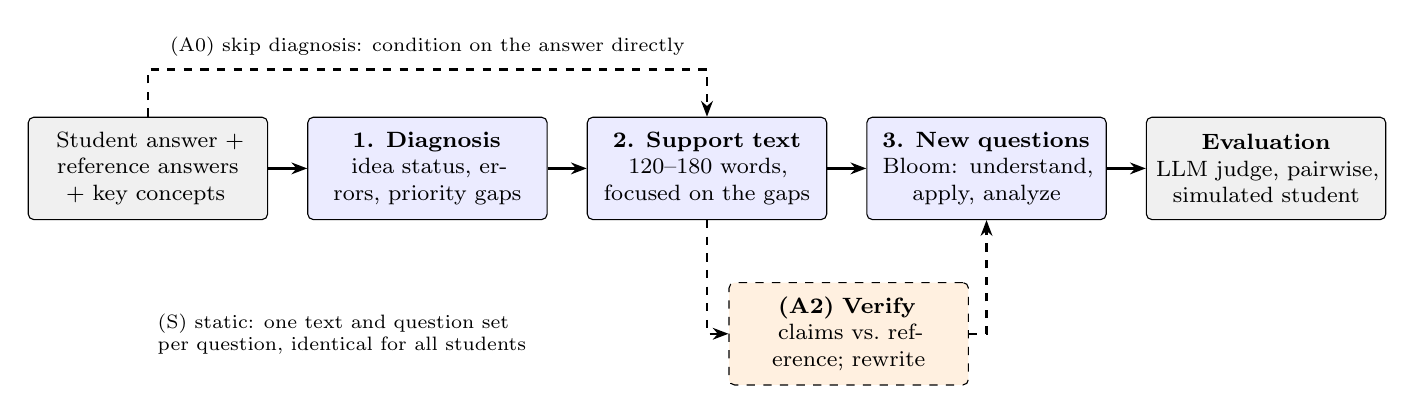
\begin{tikzpicture}[
  box/.style={draw, rounded corners=2pt, align=center, text width=29mm, minimum height=13mm, inner sep=2pt, font=\footnotesize},
  io/.style={box, fill=gray!12},
  stage/.style={box, fill=blue!8},
  opt/.style={box, dashed, fill=orange!12},
  arr/.style={-{Stealth[length=2mm]}, thick},
  darr/.style={-{Stealth[length=2mm]}, thick, dashed}]
  \node[io] (inp) at (0,0) {Student answer + reference answers + key concepts};
  \node[stage] (diag) at (3.55,0) {\textbf{1. Diagnosis}\\ idea status, errors, priority gaps};
  \node[stage] (sup) at (7.1,0) {\textbf{2. Support text}\\ 120--180 words, focused on the gaps};
  \node[stage] (qs) at (10.65,0) {\textbf{3. New questions}\\ Bloom: understand, apply, analyze};
  \node[io] (ev) at (14.2,0) {\textbf{Evaluation}\\ LLM judge, pairwise, simulated student};
  \node[opt] (ver) at (8.9,-2.1) {\textbf{(A2) Verify}\\ claims vs.\ reference; rewrite};
  \draw[arr] (inp) -- (diag);
  \draw[arr] (diag) -- (sup);
  \draw[arr] (sup) -- (qs);
  \draw[arr] (qs) -- (ev);
  \draw[darr] (sup.south) |- (ver.west);
  \draw[darr] (ver.east) -| (qs.south);
  \draw[darr] (inp.north) -- ++(0,6mm) -| (sup.north);
  \node[font=\scriptsize, above] at (3.55,1.3) {(A0) skip diagnosis: condition on the answer directly};
  \node[font=\scriptsize, align=left, anchor=west] at (0,-2.1) {(S) static: one text and question set\\ per question, identical for all students};
\end{tikzpicture}
\caption{Pipeline (A1: solid arrows). Variants: A0 conditions the generator on the answer without a diagnosis; A2 adds claim-level verification and rewriting; S gives the same material to every student; S0 uses only the teacher's reference answers.}
\label{fig:pipeline}
\end{figure*}

%% ----------------------------------------------------------------------------------------------
\section{Related Work}

\paragraph{Grading in Portuguese.} Essay-BR and ENEM-based scoring \citep{marinho2022} progressed from linguistic features to transformers, with transformers better on language-domain and cohesion competencies and all methods failing on extreme scores \citep{chalegre2026}. PT-ASAG \citep{galhardi2018} covers short answers to biology questions with a 0--3 scale; \citet{mello2025} found GPT-4 with prompt engineering competitive on unseen questions, benefiting from reasoning and rubrics in Portuguese. All of these emit a grade only.

\paragraph{Feedback generation.} \citet{filighera2022} argued that a score alone is poor guidance and released a short-answer dataset with explanatory feedback. Human feedback outperformed ChatGPT on clarity, accuracy, prioritization and tone \citep{steiss2024}, yet LLM feedback improved revision, motivation and emotions over no feedback in a randomized study \citep{meyer2024}. For Portuguese, \citet{anchieta2025} prompt several LLMs zero-shot for ENEM competencies. The common baseline is \emph{no feedback}, and the feedback derives from rubric or score rather than from an explicit conceptual diagnosis; the cycle ends at the comment.

\paragraph{Question generation.} \citet{oliveira2026} survey 132 LLM-based AQG studies. \citet{scaria2024} calibrate questions with Bloom's revised taxonomy \citep{anderson2001} across five LLMs, finding strong model variance and automatic evaluation below expert judgment; \citet{mucciaccia2025} generate and automatically evaluate Portuguese multiple-choice questions from institutional documents. Related work also explores LLM question generation and assessment more broadly \citep{maity2024,ehsan2025}. Sources are static documents, not a student's error.

\paragraph{Diagnosis and remediation.} \citet{daheim2024} separate verification from generation: a verifier locates the student's first error and the generator responds conditioned on it, yielding more focused, more correct responses with fewer hallucinations, although localization is hard even with a reference. \citet{maurya2025} propose an eight-dimension taxonomy for tutor responses and report that automatic evaluators correlate poorly with humans. Both concern English math tutoring dialogues. \citet{sonkar2024} model students with misconceptions in algebra. We instead target conceptual gaps in open Portuguese answers and produce a study text and new questions.

\paragraph{Evaluating generated text.} Hallucinations split into factuality and faithfulness errors \citep{huang2025}; both matter for study material that must be correct and aligned with a reference. LLM-as-a-judge agrees with human preferences over 80\% of the time in general chat but shows position, verbosity and self-preference biases \citep{zheng2023}; position bias depends strongly on the quality gap between candidates \citep{shi2025}. Combined with weak judge--human agreement on pedagogical dimensions \citep{maurya2025}, this motivates our controls (Section~\ref{sec:protocol}). LLM use in education carries further risks \citep{kasneci2023}.

%% ----------------------------------------------------------------------------------------------
\section{Task and Method}

\paragraph{Task.} Input: a question $q$, teacher-written reference answers $R$, key concepts $K$, and a student answer $a$. Output: a diagnosis $d$, a support text $t$, and a set of questions $Q$ aimed at the gaps in $d$. The gold grade of $a$ is \emph{never} shown to any model.

\subsection{Pipeline (A1)}
All prompts are in Portuguese (full text in the repository and Appendix~\ref{app:prompts}). Models return JSON where structured.
\begin{enumerate}\itemsep0pt
  \item \textbf{Diagnosis.} Given $(q,R,K,a)$, the model labels each key idea as \textit{present}, \textit{partial}, \textit{absent} or \textit{incorrect} with a verbatim evidence span, lists correct points and conceptual errors, selects up to three priority gaps, and estimates a 0--3 grade.
  \item \textbf{Support text.} A 120--180 word explanation that focuses strictly on the priority gaps, corrects misconceptions gently, avoids handing over the answer, and must not contradict the reference.
  \item \textbf{Questions.} Three short open questions at the \textit{understand}, \textit{apply} and \textit{analyze} levels of Bloom's revised taxonomy, aimed at the gaps, each with an expected answer.
\end{enumerate}

\subsection{Conditions}
\textbf{S0}: the teacher's reference answers as ``material'' (no LLM; no questions). \textbf{S}: one support text and question set \emph{per question}, identical for all students, generated from $(q,R,K)$ with the same word budget. \textbf{A0}: one call conditioned on $a$ producing text and questions \emph{without} an explicit diagnosis. \textbf{A1}: the pipeline above. \textbf{A2}: A1 followed by decomposing $t$ into atomic claims, labelling each \textit{supported}, \textit{general-knowledge-correct}, \textit{unsupported} or \textit{incorrect} against the reference, and rewriting $t$ (and regenerating the questions) if any claim is unsupported or incorrect.

%% ----------------------------------------------------------------------------------------------
\section{Experimental Setup}
\label{sec:setup}

\paragraph{Data.} PT-ASAG v2.0 \citep{galhardi2018}: 15 biology questions for grades 8--9 (human body, cells, genetics), 2--4 teacher reference answers and 3--6 key concepts per question, and student answers graded 0--3 (0 wrong; 1 partly correct but mostly wrong or incomplete; 2 correct with missing or wrong detail; 3 mostly correct). In the original release, only 22\% of answers were graded twice, with Pearson $r{=}0.58$. We drop duplicates and answers over 150 words and sample with a fixed seed: \textbf{E0 (diagnosis)} up to 10 answers per question$\times$grade (595 answers, balanced by grade); \textbf{pilot (generation and judging)} 4 answers per question$\times$grade for grades $\{0,1,2\}$, nested in E0 (180 answers; grade 3 answers need little remediation).

\paragraph{Models.} Diagnosis, generation and verification use GPT-4o mini \citep{openai2024mini} (temperature 0, 0.4 for generation); the judge and the grader use Gemini 2.5 Flash \citep{gemini25} (temperature 0), deliberately from a different family than the generator to limit self-preference; the simulated student is Llama 3.1 8B Instruct \citep{llama3} (temperature 0.7). All were called through the OpenRouter API on 2026-11-16 at a total cost of about US\$2.4.

\paragraph{Evaluation protocol.}\label{sec:protocol}
\textbf{E0}: quadratic weighted kappa (QWK; \citealp{cohen1968}), Spearman, MAE and accuracy of the estimated grade vs.\ gold.
\textbf{E1} (blind to condition; identical formatting): an absolute judge rates the text on 1--5 for \emph{coherence}, \emph{conceptual correctness}, \emph{faithfulness to the reference}, \emph{gap focus} (how specifically it addresses what \emph{this} student got wrong), \emph{pedagogical usefulness} and \emph{level adequacy}, and counts incorrect claims; for questions it rates alignment, clarity, gap relevance, answer correctness, and the perceived Bloom level. A pairwise judge picks the more helpful of two materials in \emph{both orders}; a win counts only if it holds in both. All generated conditions share a 120--180 word budget; actual mean lengths are reported to expose residual verbosity effects.
\textbf{E3} (exploratory): a simulated student re-answers after reading the support text (or nothing, as a control for prior knowledge); the grader scores 0--3 against the reference; gain is post$-$pre under the same grader (QWK of grader vs.\ gold on original answers: 0.60).

\paragraph{Statistics.} All contrasts are paired by item. Because the 180 items come from only 15 questions and are not independent, we report 95\% bootstrap intervals that resample \emph{questions} (5{,}000 resamples; \citealp{efron1993,field2007}) and control the family-wise error rate with Holm's procedure \citep{holm1979} over 24 comparisons (six dimensions $\times$ four contrasts) \citep[cf.][]{dror2018}. Item-level tests that ignore clustering are reported in the repository.

%% ----------------------------------------------------------------------------------------------
\section{Results}

\subsection{Diagnosis (RQ1)}
The estimated grade reaches QWK $=0.49$ (95\% CI $[0.39, 0.59]$), Spearman $0.58$, MAE $0.70$, exact accuracy $42.9\%$ and binary ($\ge 2$) accuracy $67.7\%$; per-question QWK ranges from $0.18$ to $0.78$. The diagnosis is \emph{conservative} (Table~\ref{tab:confusion}): only 11 of 145 gold-3 answers are predicted as 3, and 89 of 150 gold-2 answers are predicted as 1. The original human agreement ($r{=}0.58$, Pearson on a double-graded subset) is not directly comparable but suggests the LLM is near the human ceiling in rank correlation while being poorly calibrated, which matters because miscalibration leads to remediating ideas the student already knows.

\begin{table}[t]
\centering\small
\begin{tabular}{lcccc}
\toprule
Gold $\backslash$ Predicted & 0 & 1 & 2 & 3 \\
\midrule
0 & 85 & 63 & 2 & 0 \\
1 & 16 & 107 & 27 & 0 \\
2 & 7 & 89 & 52 & 2 \\
3 & 2 & 65 & 67 & 11 \\
\bottomrule
\end{tabular}
\caption{Confusion matrix of estimated vs.\ gold grade (E0, $n{=}595$).}
\label{tab:confusion}
\end{table}

\subsection{Individualized vs.\ static material (RQ2, RQ3)}
Table~\ref{tab:main} and Figure~\ref{fig:results}a show judge scores; Table~\ref{tab:contrasts} gives paired differences. Individualized material (A1) beats static material (S) mainly on \emph{gap focus} ($+0.80$, CI $[0.42, 1.21]$) and \emph{pedagogical usefulness} ($+0.52$, $[0.26, 0.78]$), both significant after Holm correction, and on level adequacy ($+0.12$, $[0.06, 0.18]$), with no significant difference in correctness or fidelity: individualization does not cost quality. A1 and S have the same length (159 words), so the gain is not explained by length. The effect is larger for answers with gold grade 1 and 2 (focus $+1.13$, $+0.85$) than for grade 0 ($+0.42$). The reference answers alone (S0) are far worse on every dimension, but they are also much shorter (84 words) and not written as study material, so S0 is a floor rather than evidence.

\begin{table*}[t]
\centering\small
\begin{tabular}{lrccccccc}
\toprule
Condition & Words & Coh. & Corr. & Faith. & Focus & Useful & Level & Incorr. \\
\midrule
Reference answers (S0) & 84 & 3.66 & 4.21 & 3.72 & 1.33 & 1.76 & 4.04 & 0.18 \\
\midrule
Static reinforcement (S) & 159 & 4.82 & 4.91 & 4.60 & 3.79 & 4.22 & 4.85 & 0.04 \\
Direct generation (A0) & 120 & 4.79 & 4.93 & 4.73 & 4.57 & 4.62 & 4.87 & 0.02 \\
Diagnose-then-generate (A1) & 159 & 4.92 & 4.95 & 4.74 & 4.59 & 4.74 & \textbf{4.97} & 0.01 \\
A1 + verification (A2) & 145 & \textbf{4.93} & \textbf{4.98} & \textbf{4.79} & \textbf{4.67} & \textbf{4.79} & \textbf{4.97} & 0.01 \\
\bottomrule
\end{tabular}
\caption{Mean judge scores (1--5) on 180 pilot items. Words: mean length; Incorr.: mean incorrect claims per text per the judge. Bold: best among S, A0, A1, A2 (ties both bold). 95\% intervals are in Figure~\ref{fig:results}a.}
\label{tab:main}
\end{table*}

\begin{table*}[t]
\centering\small
\begin{tabular}{lcccc}
\toprule
Dimension & A1$-$S & A0$-$S & A1$-$A0 & A2$-$A1 \\
\midrule
Coherence & $+0.11$ [0.03, 0.19] & $-0.02$ [-0.17, 0.11] & $+0.13$ [0.03, 0.24] & $+0.01$ [-0.04, 0.05] \\
Conceptual correctness & $+0.04$ [-0.03, 0.14] & $+0.03$ [-0.07, 0.12] & $+0.02$ [-0.03, 0.07] & $+0.03$ [0.01, 0.07] \\
Faithfulness to reference & $+0.14$ [-0.03, 0.31] & $+0.13$ [-0.01, 0.26] & $+0.02$ [-0.07, 0.11] & $+0.05$ [-0.04, 0.15] \\
Gap focus & $+0.80$ [0.42, 1.21]* & $+0.78$ [0.38, 1.17]* & $+0.02$ [-0.17, 0.23] & $+0.08$ [-0.05, 0.21] \\
Pedagogical usefulness & $+0.52$ [0.26, 0.78]* & $+0.39$ [0.13, 0.68] & $+0.12$ [-0.03, 0.28] & $+0.05$ [-0.06, 0.16] \\
Level adequacy & $+0.12$ [0.06, 0.18]* & $+0.02$ [-0.10, 0.12] & $+0.10$ [0.02, 0.19] & $+0.00$ [-0.03, 0.03] \\
\bottomrule
\end{tabular}
\caption{Paired differences in judge score with 95\% question-clustered bootstrap CIs. $^{*}$: Holm-adjusted $p<0.05$ over 24 comparisons.}
\label{tab:contrasts}
\end{table*}

\begin{figure*}[t]
\centering
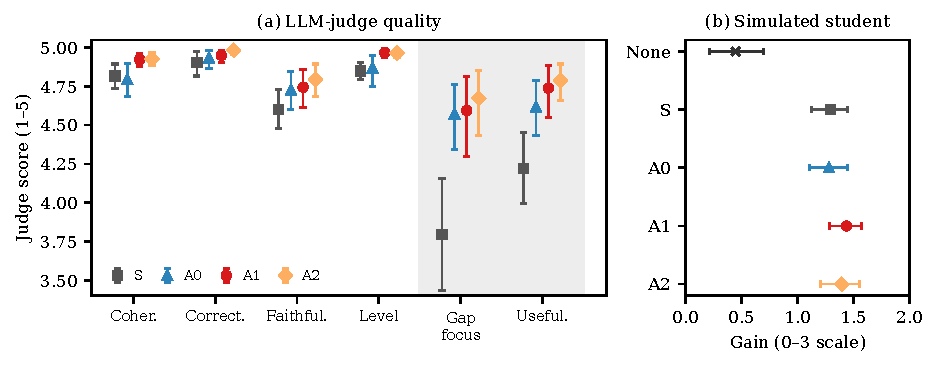
\includegraphics[width=0.78\textwidth]{figures/results.pdf}
\caption{(a) Judge scores with 95\% question-clustered CIs; shaded: dimensions where individualization helps. (b) Gain of a simulated student (0--3 scale; exploratory).}
\label{fig:results}
\end{figure*}

\paragraph{Does the explicit diagnosis help?} Largely no. Direct generation (A0) obtains almost the same focus gain over S ($+0.78$, $[0.38, 1.17]$) and a smaller usefulness gain ($+0.39$, $[0.13, 0.68]$, not significant after Holm). Comparing A1 with A0 directly, no dimension survives correction: focus $+0.02$ ($[-0.17, 0.23]$), usefulness $+0.12$ ($[-0.03, 0.28]$); coherence ($+0.13$) and level adequacy ($+0.10$) are nominally positive but not significant after Holm. \emph{Conditioning on the student's answer} thus delivers most of the benefit we can measure; the explicit diagnostic stage buys, at most, small gains in polish.

\subsection{Questions}
Generated questions (Table~\ref{tab:questions} in the appendix) are essentially always judged to have a correct expected answer ($\ge 0.99$), clear (4.8--4.9) and aligned (4.7--4.8). Gap relevance is higher for adaptive conditions (A1: $4.43$ vs.\ S: $4.19$; $+0.24$, $[0.09, 0.39]$, not in the Holm family). The requested Bloom level matches the judge's perceived level in 97--98\% of questions for all conditions; since we only requested three levels, this is a weak test of calibration.

\subsection{Verification and hallucination (RQ4)}
The verifier extracted 8.3 atomic claims per text and flagged 1.21 as unsupported or incorrect, triggering a rewrite for 73.9\% of A1 texts, yet the judge counts only $0.01$ incorrect claims per text for A1 and A2 alike (S: $0.04$; S0: $0.18$). A2 vs.\ A1 differences are small and not significant (e.g., correctness $+0.03$, $[0.01, 0.07]$). With a strong generator on a bounded school-level domain, base incorrectness is near zero (a ceiling effect), so this pilot cannot show a benefit of mitigation. Most flags are ``unsupported'' rather than ``incorrect'', which reflects the brevity of the reference answers; rewriting shortened texts (A2: 145 vs.\ A1: 159 words) and may remove helpful content.

\subsection{Judge reliability and bias}
Judge scores saturate (4.6--4.9 for most dimensions), limiting discrimination. Pairwise judging shows strong \emph{position bias} when candidates are close: the first-presented material wins only 11.5\% of non-tied judgments in A1 vs.\ S and 13.4\% in A1 vs.\ A0 (Table~\ref{tab:pairwise}); only 23--27\% of items receive the same verdict in both orders. When the quality gap is large (A1 vs.\ S0) the bias vanishes (47.9\%), in line with \citet{shi2025}. Counting only wins that hold in both orders, A1 beats A0 (18.9\% vs.\ 7.8\%) but not S (13.3\% vs.\ 9.4\%), and A1 beats A2 (21.7\% vs.\ 7.2\%), the opposite direction of the absolute scores; A1 is also longer than A2, in line with the verbosity bias of \citet{zheng2023}. Word count correlates positively with scores across conditions (Spearman 0.13--0.37). We therefore treat absolute scores with equal-length conditions as primary evidence and pairwise results as a bias diagnostic; item-level sign tests used there ignore clustering. \textbf{No human validation of the judge has been completed yet}, so all quality results are conditional on the validity of Gemini 2.5 Flash as a judge.

\subsection{Simulated student (RQ5, exploratory)}
Every material raises the simulated student's score above the no-material control ($+0.45$), by $+1.2$ to $+1.4$ (Figure~\ref{fig:results}b, Table~\ref{tab:e3} in the appendix). A1 minus S is $+0.14$ ($[-0.05, 0.33]$) and A1 minus A0 is $+0.16$ ($[0.01, 0.31]$, uncorrected); A2 minus A1 is $-0.04$ ($[-0.18, 0.06]$). Even S0 (the reference answers) obtains $+1.22$, which shows the proxy largely measures copying from the material, so it cannot establish learning benefits.

%% ----------------------------------------------------------------------------------------------
\section{Discussion}

\paragraph{What the evidence supports.} Individualized material is reliably judged more gap-focused and more useful than same-length static material, without measurable loss in coherence, correctness or fidelity, which is the central claim of our hypothesis in the classroom-realistic comparison. This supports building feedback loops that \emph{condition on the student's answer}.

\paragraph{What it does not support.} (i)~That an explicit diagnosis stage is needed: a single-call baseline matches it on the dimensions that matter. The diagnosis may still be valuable as an interpretable artifact for teachers (its QWK is moderate and conservative), which we did not evaluate. (ii)~That verification reduces hallucination: the base rate is too low here, and a same-family verifier is a weak check. (iii)~Learning gains: our proxy is confounded by copying, and no real students took part.

\paragraph{Implications.} For practitioners, the cheapest strong design is single-call personalization with a reference-grounded prompt; verification should be reserved for weaker generators or open domains. For evaluation, order-swapped judging and length control are necessary, and the judge needs human validation before pedagogical claims are made.

\section{Conclusion}
We studied closing the loop from a Portuguese short answer to individualized support text and questions, evaluated against static reinforcement. Individualization improved gap focus and usefulness at equal length without hurting quality, but explicit diagnosis and claim-level verification did not add measurable value in this pilot, and judge biases require care. Next steps are human validation of the judge, a judge from a second family, a calibrated diagnosis, weaker generators to test verification, and a study with real students.

%% ----------------------------------------------------------------------------------------------
\section*{Limitations}
\textbf{Scope.} One domain (school biology), one level (grades 8--9), 15 questions, 180 generated items; the pilot excludes gold-3 answers, so we say nothing about over-remediating correct answers. Statistics resample questions, but 15 clusters give wide intervals.
\textbf{Judge validity.} All quality results use one LLM judge (Gemini 2.5 Flash) with saturated scores, positional and length biases, and no completed human validation; GPT-4o mini generated, diagnosed and verified, so verification is same-family.
\textbf{Diagnosis.} PT-ASAG provides grades and keywords, not annotated misconceptions, so we validate the grade estimate, not the conceptual content of the diagnosis (the keyword-overlap proxy we computed is weak and omitted).
\textbf{Generation.} A single generation run per item (temperature 0.4); no repeated seeds. A0's mean length (120 words) is at the lower edge of the budget.
\textbf{Simulated student.} A proxy confounded by copying; it is not evidence of learning.
\textbf{Reproducibility.} Models were accessed through an aggregator whose underlying providers and versions may change; we release all prompts, generations and judgments, but re-running may not reproduce identical outputs.
\textbf{Language.} Prompts and data are Portuguese only; the results may not transfer to other domains or languages.

\section*{Ethical Considerations}
We use the PT-ASAG dataset (CC BY-NC-SA 4.0), which contains answers from minors, anonymized by its authors; we collected no new data and did not recruit students, and our released outputs include only short excerpts under the same license. LLM-generated study material may contain errors and could mislead students; any deployment should keep a teacher in the loop and not use these systems for high-stakes decisions. Tone (encouraging language) can also affect students; we did not study it. The experiments cost about US\$2.4 in API usage.

\section*{Acknowledgments}
We used an AI assistant to draft code, analysis scripts and parts of this manuscript; the authors are responsible for the content and must verify all claims, numbers and references before submission.

\bibliography{references}
\bibliographystyle{acl_natbib}

\appendix
\section{Appendix}
\label{app:prompts}

\subsection{Prompts}
All prompts are in Portuguese (see \texttt{src/pln/prompts.py}). The judge rubric states: \emph{evaluate independently of length or style; a longer or better-written text is not better per se}. Gap focus is defined as ``how specifically the text addresses what \emph{this} student got wrong or omitted (1 = generic, ignores the student's error; 5 = attacks exactly their gaps without repeating what they know)''. The pairwise prompt asks which material would help \emph{this} student most while remaining correct and faithful to the reference, ignoring length and style.

\subsection{Additional tables}
\begin{table}[h]
\centering\small
\begin{tabular}{lc}
\toprule
Material given to simulated student & Gain [95\% CI] \\
\midrule
No material & $+0.45$ [0.21, 0.69] \\
Reference answers (S0) & $+1.22$ [0.93, 1.43] \\
Static reinforcement (S) & $+1.29$ [1.13, 1.44] \\
Direct generation (A0) & $+1.28$ [1.11, 1.44] \\
Diagnose-then-generate (A1) & $+1.44$ [1.28, 1.57] \\
A1 + verification (A2) & $+1.39$ [1.21, 1.56] \\
\bottomrule
\end{tabular}
\caption{Simulated-student gain (post$-$pre, 0--3 scale) with question-clustered 95\% CIs.}
\label{tab:e3}
\end{table}

\begin{table}[h]
\centering\footnotesize
\begin{tabular}{lcccc}
\toprule
Condition & Alignment & Clarity & Gap relevance & Bloom match \\
\midrule
Static reinforcement (S) & 4.67 & 4.84 & 4.19 & 0.98 \\
Direct generation (A0) & 4.73 & 4.88 & 4.31 & 0.97 \\
Diagnose-then-generate (A1) & 4.80 & 4.82 & 4.43 & 0.97 \\
A1 + verification (A2) & 4.80 & 4.84 & 4.46 & 0.98 \\
\bottomrule
\end{tabular}
\caption{Judge scores for generated questions (1--5) and agreement of requested vs.\ perceived Bloom level.}
\label{tab:questions}
\end{table}

\begin{table*}[h]
\centering\small
\begin{tabular}{lcccc}
\toprule
Pair ($x$ vs $y$) & $x$ wins both & $y$ wins both & Order-inconsistent/tie & 1st-position wins \\
\midrule
A1 vs A0 & 18.9\% & 7.8\% & 73.3\% & 13.4\% \\
A1 vs S0 & 66.7\% & 6.7\% & 26.7\% & 47.9\% \\
A1 vs S & 13.3\% & 9.4\% & 77.2\% & 11.5\% \\
A2 vs A1 & 7.2\% & 21.7\% & 71.1\% & 31.4\% \\
\bottomrule
\end{tabular}
\caption{Pairwise judgments in both orders (180 items per pair). A win counts only if the same material wins in both orders. ``1st-position wins'': share of non-tied verdicts won by the material shown first (50\% = no position bias).}
\label{tab:pairwise}
\end{table*}

\subsection{Qualitative example}
Question: \emph{What is the difference between animal and plant cells?} Student answer (gold grade 1): \emph{``na celula vegetal tem cloroplasto e na animal n\~ao''} (``plant cells have chloroplasts and animal cells do not''). The diagnosis's priority gaps were: difference in shape, presence of the cell wall, and its composition (cellulose). A1 opens by acknowledging the correct chloroplast point and then addresses exactly those gaps with an everyday analogy (``imagine the wall of a building''), scoring 5/5 on gap focus and usefulness. The static text S gives a correct and fluent general description of shape, wall and cellulose, without referencing the student's answer, and scored 1/5 on gap focus and 3/5 on usefulness. A0 also acknowledges chloroplasts, but adds content not in the reference answers (vacuoles).

\end{document}
